Ci-dessous, un graphe montre la différence entre:
\begin{itemize}
    \item le coût obtenu, pour un certain epsilon et pour une certaine légère modification de la demande, via la procédure présentée à la question 4 et
    \item le coût obtenu en résolvant complètement le problème avec les données initiales modifiées.
\end{itemize}

Sur le graphe, la différence est normalisée en pourcentage par rapport au résultat obtenu via la seconde méthode. Chaque point vaut:
\begin{equation*}
\mathrm{difference} =
\frac{\left|\mathrm{resultat}_\mathrm{dual} - \mathrm{resultat}_\mathrm{reecriture}\right|}{\mathrm{resultat}_\mathrm{reecriture}} \times 100 
\end{equation*}
 
\begin{figure}[h]
    \centering
    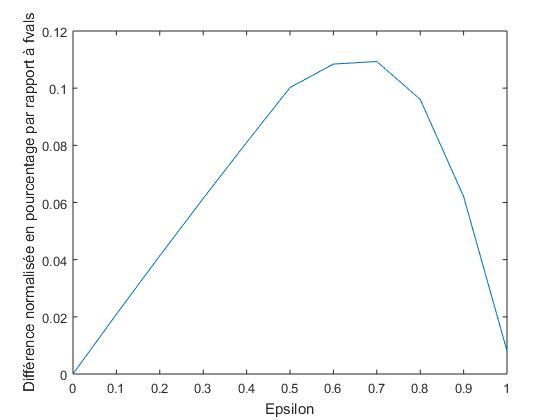
\includegraphics[width=0.8\textwidth]{graphes/graphq5.jpg}
    \caption{Graphe de la différence normalisée entre la solution du problème non perturbé modifié d'un epsilon à l'aide du dual, et la solution du problème perturbé}
    \label{fig:q5}
\end{figure}

La différence entre les deux méthodes dépasse à peine les 0,1\%, ce qui est négligeable à l'échelle utilisée ici. La procédure présentée à la question 4 est donc suffisante.
